\documentclass[11pt]{article}
\usepackage[review]{acl}
\usepackage{times}
\usepackage{latexsym}
\usepackage[T1]{fontenc}
\usepackage[utf8]{inputenc}
\usepackage{microtype}
\usepackage{inconsolata}
\usepackage{booktabs}
\usepackage{tabularx}
\usepackage{adjustbox}
\usepackage{pgfplots}
\pgfplotsset{compat=1.18}
\usepgfplotslibrary{groupplots}
\usetikzlibrary{calc}
\newcolumntype{L}{>{\raggedright\arraybackslash}X}
\newcolumntype{R}{>{\raggedleft\arraybackslash}X}

\title{Agents as System 2: Building System 1 Primitives for Agentic Systems}
\author{Anonymous ACL submission}

\begin{document}
\maketitle

\begin{abstract}
Agentic systems often use a reasoning model both as the controller and as the worker that performs repeatable judgements, spending its compute on work a fast classifier could do. We argue that such classifiers should act as the agent's System 1, with the agent as System 2 that builds, monitors and updates them. A fine-tuned classifier could fill this role, but its decision rule is hidden in its weights, and changing it means relabelling and retraining. A natural-language (NL) classifier, composed of questions put to a small judgement model such as Jev, can be read and edited by the agent and its user. We first ask whether agent-built NL classifiers are as effective as fine-tuned ones: given the same training labels, an Opus builder matches or beats RoBERTa fine-tuned on them on all six of our tasks, and its classifiers keep their scores, unchanged, when three other System 1 models answer their questions, including one forty times as expensive. We then study the more common case for an agent, where no labelled data exists: the agent receives a brief description and unlabelled data, and spends a budget of a simulated user's time on labels and on questions about the definition. With 100 points, about 50 labels, it beats zero-shot wherever the user has something to teach, and on two tasks it beats an encoder fine-tuned on twenty times as many labels. The best strategy, chosen on a validation split, depends on where the missing knowledge lies: labels turned into rules suffice when the definition shows in the text or in the labels, and fail when it is a private policy that must be probed with questions. Builder capability matters at every step: Sonnet trails Opus, Haiku trails both, and Haiku gains nothing from plentiful labels, suggesting that acting on evidence, more than access to it, limits what an agent can build.
\end{abstract}

\section{Introduction}

The field of Natural Language Processing has been driven by the rise of ever more capable models, and intelligent agentic systems that communicate in natural language are becoming a reality \citep{yao2023react,schick2023toolformer,wang2024survey}. In these systems a highly capable model that can reason serves as the controller: it plans, calls tools, and decides what to do next. Often, however, the same model also serves as the worker, performing repeatable, well-understood tasks such as routing a message, checking whether a record matches a filter, or deciding whether an email needs a reply, one input at a time. Each such call spends the compute and latency of a reasoning model, which results in a waste of compute and of intelligence.

Human cognition offers a parallel in its two modes of thinking \citep{kahneman2011thinking}: System 1, fast and automatic, and System 2, slow and deliberate. A new task first takes the effort of System 2; with practice, System 1 learns to do it, while System 2 monitors it and steps in when it errs. The distinction has been proposed as a template for AI \citep{bengio2019system2,booch2021thinking}, but most agentic systems never make the hand-off: the reasoning model performs every judgement itself, however often it recurs.

The recent resurgence of classification models such as Jev \citep{typesafe2026} offers an interesting option for the role of System 1 in an agentic system. They answer a precisely stated question about an input, a choice among options or a yes/no judgement, with a typed answer and a probability, quickly, cheaply and consistently. Encoding a classifier in natural language rather than in parameters, as traditional classifiers fine-tuned from encoders such as BERT and RoBERTa do \citep{devlin2019bert,liu2019roberta}, is a clear advantage for a system controlled by an agent. Both the agent and the user can interpret the rules of such a \textbf{natural-language (NL) classifier}, build and iterate on it, and the system needs no traditional training loop. Put succinctly: the agent can write a decision policy for a classifier, the user can read it, and a change of policy is an edit to a sentence.

In this paper, we explore whether a highly capable model given an NL classifier as a subroutine can act as System 2: interpret labels and user feedback to build a classifier that performs its repeatable judgements. This translates into three research questions:

\begin{itemize}
\item \textbf{RQ1:} given training labels, can an agent build NL classifiers as effective as a supervised classifier trained on the same labels?
\item \textbf{RQ2:} without labelled data, how well can an agent build them from a task description, unlabelled data and a short user interview?
\item \textbf{RQ3:} which interview strategies work well, and does the answer depend on the task?
\end{itemize}

We find that a frontier model can use an NL classifier effectively as a System 1 routine. On six classification tasks, a frontier model (Claude Opus 5.5) using Jev matches or beats a fine-tuned RoBERTa when both are given a full labelled set. With a budget equivalent to about 50 labels of a simulated user's time, it beats zero-shot wherever the user has something to teach, and on two tasks beats RoBERTa fine-tuned on twenty times as many labels. The best strategy depends on where the missing knowledge lies: following the classifier's uncertainty and turning errors into rules works when the definition is in the text or shows in the labels, and fails when it is a private policy the agent must discover by asking. Doubling the budget helps most where the policy is private and least where the builder already knows the scheme. We also find that other available options can play the role of System 1 with little difference in accuracy, but the System 2 model matters: with the same strategy and budget, Sonnet 5.5 builds worse classifiers than Opus 5.5, and Haiku 4.5 worse than both.

We start with a review of related work in Section 2. Section 3 formulates budgeted building with a simulated user, and Section 4 describes the toolkit and builder. We describe the experiments in Section 5 and discuss the results in Section 6. Finally, we conclude with a discussion of monitoring and updating deployed classifiers as part of a functioning agentic system in Section 7, followed by the limitations of this study.

\section{Related Work}

\textbf{Agents and the cost of reasoning.} Language agents use a reasoning model to plan, call tools and act \citep{yao2023react,schick2023toolformer,wang2024survey}. Several lines of work reduce the cost of such systems by sending easy inputs to cheaper models, through cascades and routers between language models \citep{chen2023frugalgpt,ong2024routellm}, or by distilling a large model's behaviour into a small one \citep{hsieh2023distilling}. Dual-process architectures pair a fast and a slow component explicitly \citep{bengio2019system2,booch2021thinking,lin2023swiftsage}. In these systems the fast component is a smaller generator or a trained network. We instead make it a classifier whose definition is text, which the slow component writes and can later revise.

\textbf{Classifiers defined in natural language.} Zero-shot classification casts labels as natural-language hypotheses or prompts \citep{yin2019benchmarking,schick2021exploiting}, and instruction-tuned models follow task definitions written for people \citep{mishra2022cross}. Natural-language explanations and labelling functions have also been used to train conventional classifiers \citep{hancock2018training,ratner2017snorkel}. In our setting the definition is not a means of producing training data but the classifier itself, executed by a small judgement model such as Jev \citep{typesafe2026}.

\textbf{Prompt optimisation.} Methods that search over instructions, such as APE, ProTeGi, OPRO and DSPy, improve a prompt against a labelled set \citep{zhou2023ape,pryzant2023automatic,yang2024opro,khattab2024dspy}. Our setting with every training label is closest to this work, with a general agent in place of a fixed search procedure. Without labels, these methods have nothing to optimise against, and the builder must first acquire the evidence.

\textbf{Active learning, machine teaching and elicitation.} Active learning chooses which examples a person should label \citep{settles2009active}, and some variants also ask the annotator about features, at a different cost \citep{raghavan2006active,druck2009active}. Machine teaching shifts the focus to how a person transfers a concept to a learner \citep{simard2017machine}. Closest to our setting, language models have been used to elicit a user's preferences by asking open questions as well as for labels \citep{li2023eliciting}, motivated by the ambiguity of tasks specified in a few words \citep{tamkin2023task}. We study the same trade-off between labels and questions when the learner is an agent that must also encode what it learns in a classifier, and compare strategies for it on tasks where the missing knowledge lies in different places.

\textbf{Few-shot text classification.} With a few dozen labels, contrastive fine-tuning of sentence encoders is a strong baseline \citep{tunstall2022setfit}. We compare against RoBERTa \citep{liu2019roberta} fine-tuned on 50 labels, about what our budget buys, and on every training label.

\section{Task Formulation}

We model building as an interaction between an agent, the \textbf{builder}, and a \textbf{user} who needs a classifier. We simulate the user with an agent that holds two things the builder cannot see: a \textbf{guideline} that states the definition they have in mind, and the gold \textbf{labels}. The builder's output is an NL classifier: questions and option descriptions, combined into one of a few fixed structures (Section 4). As part of the process the builder has access to the unlabelled examples and is able to run different versions of the classifier.

\textbf{Building with labels.} In the supervised setting (RQ1), the builder receives all gold labels and does not interact with the user.

\textbf{Building from a user interview.} In the budgeted setting (RQ2 and RQ3), the builder starts with no labels and a budget of 100 points of the user's time. It can ask the user to \textbf{label} a pool record, which costs 2 points, or it can \textbf{ask} a question, which the user answers and prices by a fixed rubric meant to reflect the effort of answering:

\begin{itemize}
\item \textbf{2 points:} a question about a single record or type of message, or a yes/no fact;
\item \textbf{5 points:} a targeted question about a rule or a group of messages;
\item \textbf{10 points:} an open-ended question that needs a view across many examples, such as ``what are the main confusions?'', answered in summary.
\end{itemize}

A message can contain multiple questions, and their costs are added up. Requests that would exceed the budget are refused, and points left over do not affect the score.

\textbf{The simulated user.} A language model plays the user (Claude Opus 5.5 \citep{anthropic2026}). A user who wrote a guideline and a user who labelled the data know different things: annotators settle cases the guideline does not cover and apply it more loosely or strictly in places. We want the user's answers to agree with the labels the builder is scored on, so before any run the same model reads each task's labelled pool through search tools and writes a private note of at most about 1,200 words on how the labels apply the guideline, including where they depart from it and how consistent they are. When answering, the user sees the task description, the guideline, this note, the records a question mentions and a fixed labelled sample of 150 pool records, and is told that where the note and the guideline differ, the note is right. It prices each message by the rubric above and answers as a busy domain expert would: only what is asked, without reciting the guideline or volunteering rules, and in summary for open-ended questions. Requests for labels always return the gold labels. An earlier simulated user without the note drifted towards the guideline; Section 6.3 shows how that changed the results.

\textbf{Evaluation.} Each task also has a validation split, used to tune the baselines and to choose among strategies (Section 5.3), and a sealed \textbf{test} split; the builder never sees the labels of either. After its first draft and after every revision it keeps, the builder saves a \textbf{snapshot} of its classifier together with its own estimate of the score. After the run we score every snapshot on the test set. The final snapshot defines the run's result, and the earlier ones trace how the score develops as points are spent. Builders work in isolation and cannot read the labelled data, the task files or other runs (Section 4).

\section{System}

The system has three parts: a System 1 model that answers questions, a classifier format that composes those questions, and a skill that gives a coding agent the tools to write, run and revise classifiers.

\subsection{System 1: Jev}

Jev \citep{typesafe2026} answers questions about a \textbf{state}, a piece of text such as a message or a dialogue. A question is one of three types: a \textbf{choice} among up to 255 options, each with an optional description, which returns a probability for every option; a \textbf{yes/no} question, which returns the probability of yes; and a \textbf{score} on an ordered scale of up to ten levels, which returns a distribution over the levels. Its instructions and option descriptions can be structured, with definitions, inclusions and exclusions. One request can hold several questions about the same state, and the answers are deterministic.

\subsection{NL classifiers}

An NL classifier holds the static part of a Jev request: a template that renders the input as a state, and one or more questions. It takes one of five shapes:

\begin{itemize}
\item \textbf{flat choice:} one choice question whose options are the classes;
\item \textbf{option map:} a choice with more options than classes, mapped many to one, where each class receives the summed probability of its options;
\item \textbf{two-level:} a router question picks a group of classes and a second question picks a class within it, both asked in one request, so that a wrong group can be outweighed;
\item \textbf{criteria:} several yes/no questions combined by a rule, for a policy that is a conjunction of tests;
\item \textbf{ensemble:} the average of several classifiers, usually rewordings of one.
\end{itemize}

Any shape that yields class probabilities can also store a decision threshold. Running a classifier returns, for each record, the predicted class, the class probabilities, the most likely option and a \textbf{margin}, how far the prediction is from flipping. A classifier is only text and a few structural fields, so the user can read it, and changing a rule means editing a sentence. Because its questions are plain text, other System 1 models can answer them too (Section 5.4).

\subsection{The builder}

The builder is a general-purpose coding agent with shell access, given a run directory and the classifier-builder skill, a document it reads at the start of the run. The run directory holds the task description and class names, the unlabelled pool, the labels bought so far, and a journal the builder keeps. The skill explains the budget, the classifier format and how Jev behaves: it judges meaning better than surface patterns, does better with concrete options than with abstract ones, and can flip near-tied records on small rewordings. It then sets out a generic workflow. The builder reads the pool, writes a first draft from the description, lists what it does not know and buys the cheapest evidence that resolves it, and revises, saving a snapshot after each kept revision. It stops when nothing left to buy would change its predictions. The skill also warns that the user's answers about edge cases can disagree with their own labels, and that labels chosen because they are hard give a biased estimate of accuracy. A strategy replaces the middle of this workflow (Section 5.2). The tools are:

\begin{center}\small
\begin{tabularx}{\linewidth}{lLl}
\toprule
Tool & What it does & Cost \\
\midrule
Run & run a classifier on the pool or on bought labels & free \\
Label & ask the user for the labels of pool records & 2 each \\
Ask & ask the user a question & 2, 5 or 10 \\
Score & score on bought labels, with a 90\% interval & free \\
Uncertain & list the records with the smallest margin & free \\
Sample & pick records at random or spread over the options & free \\
Diff & compare two versions on the pool and bought labels & free \\
Threshold & fit a decision threshold for a class & free \\
Snapshot & save a version with an estimate of its score & free \\
\bottomrule
\end{tabularx}
\end{center}

Running classifiers costs the builder nothing, since Jev calls are cheap and cached; only the user's time is budgeted. Two further tools serve particular settings: the rules-only constraint adds a check that flags any six-word run shared by the definition and the pool, and the boundary strategy of Section 6.1 adds one that lists low-margin records by class pair and gives a verdict on each revision. With every training label, the labels file simply holds them all, and the same tools report per-class scores, confusions and scores on subsets.

Each builder first claims its run and receives a token that every command spending points or saving a snapshot requires, so concurrent builders cannot spend each other's budget. A hook checks every tool call before it runs and refuses reads of the labelled data, the task files, other runs and the simulated user's source, as well as web access beyond the TypeSafe documentation. Refusals are returned to the builder and logged.

\section{Experiments}

\subsection{Tasks and data}

We pick six tasks by where the knowledge the builder lacks lives: in the text, in a definition only the user holds, or nowhere the user can supply (Table 1). Three tasks judge single messages and three judge conversations, the setting that motivates this work.

\begin{table*}[t]
\centering\small\setlength{\tabcolsep}{3.5pt}
\begin{tabularx}{\textwidth}{lLLRLL}
\toprule
Task & Input & Classes & Pool / val / test & Zero-shot (test) & Where the missing knowledge lives \\
\midrule
Banking77 intents \citep{casanueva2020efficient} & a customer message & 77 & 1,000 / 200 / 3,080 & 80.2\% acc & mostly in the text \\
Banking77 routing & a customer message & 6 teams & 1,000 / 200 / 3,080 & 73.7\% acc & a private mapping of intents to teams \\
Hate speech (HatEval \citep{basile2019semeval}) & a tweet & 2 & 1,000 / 200 / 1,766 & 0.741 macro-F1 & an unstated annotation policy \\
Persuasion strategy (Persuasion for Good \citep{wang2019persuasion}) & a persuader's message with the dialogue so far & 18 & 1,002 / 224 / 1,517 & 0.455 macro-F1 & a scheme defined by its annotation manual \\
Donation outcome (Persuasion for Good) & a whole charity-solicitation dialogue & 2 & 500 / 100 / 417 & 0.733 macro-F1 & nowhere: the label is a fact \\
Deal reached (CraigslistBargain \citep{he2018decoupling}) & a price negotiation without the formal offer and accept events & 2 & 1,000 / 200 / 582 & 0.889 macro-F1 & nowhere: a near-ceiling control \\
\bottomrule
\end{tabularx}
\caption{tasks. Zero-shot is the classifier built from the task description and class names alone.}
\label{tab:1}
\end{table*}

\textbf{Banking77 intents} asks for one of 77 fine-grained intents of a customer message to a bank. The intent names are informative, and the difficulty is separating near-synonyms such as a pending card payment and a pending transfer. \textbf{Banking77 routing} labels the same messages with one of six support teams by a private mapping from intents to teams, which includes some counter-intuitive assignments. \textbf{Hate speech} (HatEval, SemEval-2019 Task 5, English, via TweetEval \citep{barbieri2020tweeteval}) labels tweets under a policy restricted to hate against women and immigrants, while the builder is told only that the labels follow ``our annotation policy for hate speech''.

The three conversation tasks come from an accuracy and calibration benchmark of Jev \citep{typesafe2026b}. In \textbf{persuasion strategy} the user's definitions are the point: the builder must learn, for example, that citing the charity's track record is a credibility appeal rather than a logical one. In \textbf{donation outcome} no definition decides whether the persuadee gave, so any gain has to come from labels. \textbf{Deal reached} is nearly solved zero-shot and tests whether builders know when to stop. We exclude the benchmark's fourth task, yes/no answers to Amazon product questions \citep{mcauley2016addressing}, on which Jev scores below the majority class.

We write each task's description and private guideline from the corpus's annotation instructions, keeping the description as brief as a request to an assistant. Splits are stratified, deduplicated and fixed by seed. Banking77 draws the pool and validation split from the official training split and tests on the official test set. HatEval's official test set is shifted from its training distribution, so we draw all three splits from it, and our scores are not comparable with published HatEval results. Persuasion strategy is split by dialogue, and deal reached tests on the corpus's validation split. Public datasets may let the builder recall the labels; routing, whose mapping is our own, measures what the builder has to acquire.

\subsection{Builders and strategies}

The main experiments use Claude Opus 5.5 \citep{anthropic2026}, and we repeat the key cells with Claude Sonnet 5.5 and Claude Haiku 4.5 to measure how much building depends on the builder's capability. Builders run headlessly through the Claude Agent SDK at high reasoning effort, with one prompt template for every task and model, and every session transcript is kept. A pilot on Banking77 intents and hate speech ran Opus builders interactively.

A \textbf{strategy} is a one-page instruction that replaces the skill's generic building step. We compare six:

\begin{center}\small
\begin{tabularx}{\linewidth}{lL}
\toprule
Strategy & Summary \\
\midrule
Free & The skill's generic workflow only. \\
Uncertainty & Buy the records with the smallest margin between the top two classes in small batches, and revise after each batch. \\
Uncertainty + rules & As above, but turn errors into general rules, and test any rule that moves many pool predictions with a label on a moved record. \\
Policy first & Ask the user about the main policy decisions, build a classifier that mirrors the answers, then calibrate with random labels. \\
Policy, labels first & Ask policy questions, then check the draft against random labels before testing edge cases, and follow labels where they contradict the user. \\
Interview, lean & Read the pool and mark each phenomenon inferable or private; ask only about the private ones; spend the rest on whatever labels the builder chooses. \\
\bottomrule
\end{tabularx}
\end{center}

The pilot also tried a category-by-category audit, a committee of three classifiers, a triage step and policy + rules; none beat the best strategy on either pilot task. A fuller interview, with fixed allowances for questions, coverage labels and a check set, ran only with the earlier simulated user and is not reported. Any strategy can run under the \textbf{rules-only constraint}, under which labels are evidence for rules and never enter the classifier: the definition may contain no text from a pool record, and a rule is kept only if it holds on records beyond the one that prompted it. The lean interview runs under it.

\subsection{Settings}

\textbf{All labels (RQ1).} The builder receives the gold label of every training record and no budget. For the Banking77 tasks and deal reached this is the full training split (9,792 messages and 4,947 negotiations); for the other three it is the pool, which is all their labelled data outside the validation and test splits. The labels do not fit in context, so the builder queries them through tools (per-class scores, frequent confusions, scores on subsets), splits them into a building set and a development set of its choosing, and estimates its score on the latter. It gets no strategy; the prompt asks only that it hold out a development set, work from per-class scores and confusions, and state general rules rather than copy training records. We run Opus on all six tasks and Sonnet and Haiku on three, one run each.

\textbf{User interview (RQ2 and RQ3).} The \textbf{cross-strategy} grid runs Opus with all six strategies on all six tasks, three runs per cell. We score every final classifier on the validation split as well as the test split, choose each task's strategy by its mean validation score, and report the test score of that choice; Table 6 reports every cell. The \textbf{cross-model} grid repeats the chosen strategy with Sonnet and Haiku on Banking77 intents, hate speech and persuasion strategy, three runs each. The \textbf{budget} grid runs Opus at 50 and 200 points on Banking77 intents, routing, hate speech and persuasion strategy with uncertainty + rules and policy with labels first, three runs each, and we ran the rules-only constraint in five runs matched to uncertainty runs. Every reported run that asked the user a question uses the simulated user of Section 3; runs that only bought labels do not depend on the simulated user, and some were kept from earlier rounds.

\subsection{System 1 models}

Jev answers every question while building, at \$0.042 per million input tokens. To test whether the classifiers depend on Jev, we run them unchanged on three other System 1 models. Perplexity's decision model \citep{perplexity2026} takes Jev's request format directly. GPT-6 Luna \citep{openai2026}, a small general model at low reasoning effort, and Claude Sonnet 5 \citep{anthropic2026}, a large one without thinking, receive each question as a prompt with the options and their descriptions and return one option with a confidence. The other options share the remaining probability, so every classifier shape runs unchanged.

\subsection{Baselines and metrics}

Our baselines are the \textbf{zero-shot} classifier, built from the description and class names alone; the builder's \textbf{first draft}, its first saved snapshot; and RoBERTa-base \citep{liu2019roberta} fine-tuned on the same labels as the all-labels builder, with the epoch chosen on the validation split. On the cross-model tasks we also fine-tune RoBERTa on 50 stratified labels, about what a 100-point builder buys, over three seeds.

We report test accuracy on Banking77 and macro-F1 elsewhere, for the final snapshot. Jev is deterministic, so the variance between runs comes from the builder, and we repeat the main cells three times. We compare two classifiers with an exact McNemar test on paired predictions. We compare groups of runs with a paired bootstrap over test records (2,000 resamples), which captures test-set noise, and with an exact permutation test over run scores, which captures run-to-run variance but cannot go below p = 0.05 with three runs per group. We log the cost of every run: the builder's API calls, the simulated user's, and the System 1 calls made while building.

\section{Results}

\subsection{RQ1: building with every label}

\textbf{With every label, an Opus builder matches or beats RoBERTa fine-tuned on the same labels on all six tasks} (Table 2). On hate speech and persuasion strategy, with about a thousand labels, both larger builders beat RoBERTa by 0.02--0.05 macro-F1. With ten thousand labels, Opus edges RoBERTa on both Banking77 tasks but stays below published full fine-tuning on intents (94.1\%), and on deal reached the two are level with zero-shot. These are single runs, so margins under a point amount to parity. Donation outcome is the exception to more labels helping: both learners end below zero-shot, because 500 labelled dialogues teach cues that do not hold on the test set.

\begin{table*}[t]
\centering\small\setlength{\tabcolsep}{3.5pt}
\begin{tabularx}{\textwidth}{lRRRRRRRR}
\toprule
Task & Labels & Zero-shot & RoBERTa, 50 labels & Opus, 100 pts & RoBERTa, all labels & Opus, all labels & Sonnet 5.5, all labels & Haiku 4.5, all labels \\
\midrule
Banking77 intents (acc) & 9,792 & 80.2 & 18.1 & 86.3 & 91.1 & \textbf{91.9} & 91.3 & 79.4 \\
Banking77 routing (acc) & 9,792 & 73.7 & --- & 94.0 & 96.8 & \textbf{97.5} & --- & --- \\
Hate speech (macro-F1) & 1,000 & 0.741 & 0.635 & 0.818 & 0.780 & \textbf{0.823} & 0.803 & 0.729 \\
Persuasion strategy (macro-F1) & 1,002 & 0.455 & 0.137 & 0.613 & 0.582 & 0.616 & \textbf{0.629} & 0.486 \\
Donation outcome (macro-F1) & 500 & \textbf{0.733} & --- & 0.725 & 0.675 & 0.680 & --- & --- \\
Deal reached (macro-F1) & 4,947 & 0.889 & --- & 0.886 & 0.889 & \textbf{0.896} & --- & --- \\
\bottomrule
\end{tabularx}
\caption{test scores with Jev as System 1. Labels is the number of training labels in the all-labels setting. Opus at 100 points is the mean of three runs with the strategy chosen on the validation split (Table 4). RoBERTa with 50 labels averages three seeds; all-labels cells are single runs.}
\label{tab:2}
\end{table*}

\textbf{Using the labels takes a capable builder.} Sonnet comes within 0.6 points or 0.02 macro-F1 of Opus and is ahead on persuasion strategy. Haiku gains nothing: its all-labels classifiers score no better than its budgeted ones, and in all three runs its final classifier is its first draft. It read and split the labels but did not turn them into revisions, while Opus saved three to six improving snapshots. The failure is not one of judging its own classifier: every builder, Haiku included, estimated its score on its development set to within 0.035 of the test score.

\textbf{The builders converged on the same loop.} Without being told, the larger builders wrote a first draft from the description and a sample, ran it on the building set, and revised by rewriting the descriptions of the options with the most errors. Seven of the nine Opus and Sonnet classifiers use options finer than the classes, mapped many to one: 13 options for the two hate speech classes, 28 for the 18 persuasion strategies, and about 100 intent-level options with a learned team map on routing. Eight of the twelve classifiers are ensembles of two to four wordings, and none reproduces a training record. Builders mostly stopped when the remaining errors looked like disagreement among the labels; the persuasion builder, for instance, found ``Great!'' labelled almost at random as thanks, praise or acknowledgement.

\textbf{Revisions trade errors near the decision boundary.} Comparing consecutive snapshots on the test set after the runs, a correct record with a margin below 0.1 was broken by the next revision 32\% of the time, against 0.7\% for a record with a margin of 0.6 or more, and several late revisions were near-even trades on the builders' own building sets. We turned this into a strategy: read the low-margin records by class pair and either state a rule that separates the pair or declare it ambiguous, check each confident error against the nearest record labelled the other way, and keep a revision only if its fixes minus breaks exceed 2$\surd$(fixes + breaks). The strategy is level with no strategy on average (Table 3). Its one clear effect is on donation outcome, where the noise check rejected the over-tuning that had lowered the unguided run.

\begin{table}[t]
\centering\small
\begin{adjustbox}{max width=\linewidth}
\begin{tabular}{lrr}
\toprule
Task (macro-F1) & No strategy & Boundary strategy \\
\midrule
Hate speech & \textbf{0.823} & 0.814 \\
Persuasion strategy & \textbf{0.616} & 0.609 \\
Donation outcome & 0.680 & \textbf{0.719} \\
Deal reached & 0.896 & \textbf{0.902} \\
Mean & 0.754 & \textbf{0.761} \\
\bottomrule
\end{tabular}
\end{adjustbox}
\caption{Opus all-labels builders without a strategy and with the boundary strategy, one run each. Each per-task difference is within the noise of a single run.}
\label{tab:3}
\end{table}

\subsection{RQ2: building from a user interview}

\textbf{Without labels, Opus beats zero-shot wherever the user has something to teach} (Table 4). On Banking77 intents, routing, hate speech and persuasion strategy, the final classifier with the strategy chosen on validation beats zero-shot in every run, by 6.1 points, 20.3 points, 0.077 and 0.158 on average, closing 52\%, 85\%, 94\% and 98\% of the gap to the all-labels builder. With a budget worth about 50 labels, it beats RoBERTa fine-tuned on all 1,000 on hate speech and persuasion strategy in every run, while RoBERTa fine-tuned on 50 labels is far behind on every task. The encoder needs labels to learn what the classes mean; the builder brings that knowledge and uses labels to learn where the user draws the lines.

\begin{table*}[t]
\centering\small\setlength{\tabcolsep}{3.5pt}
\begin{tabularx}{\textwidth}{lLLRRR}
\toprule
Task & Metric & Strategy (chosen on validation) & Zero-shot & First draft & Final (100 pts) \\
\midrule
Banking77 intents & acc & Free & 80.2 & 84.1 & 86.3 (85.9--86.6) \\
Hate speech & macro-F1 & Uncertainty + rules & 0.741 & 0.768 & 0.818 (0.816--0.821) \\
Persuasion strategy & macro-F1 & Uncertainty + rules & 0.455 & 0.606 & 0.613 (0.606--0.626) \\
Banking77 routing & acc & Policy, labels first & 73.7 & 92.9 & 94.0 (92.6--94.9) \\
Donation outcome & macro-F1 & Uncertainty & 0.733 & 0.713 & 0.725 (0.710--0.734) \\
Deal reached & macro-F1 & Uncertainty + rules & 0.889 & 0.864 & 0.886 (0.865--0.908) \\
\bottomrule
\end{tabularx}
\caption{Opus builders with 100 points, test set, three runs per task with the strategy whose mean validation score was highest. First draft is the mean score of each run's first snapshot. Ranges give the lowest and highest run.}
\label{tab:4}
\end{table*}

\textbf{Where the gain comes from depends on the task.} On Banking77 intents, the first draft, written from the description and the pool, closes 3.9 of the 6.1 points, and on persuasion strategy first drafts already reach 0.600--0.611 from the builder's knowledge of the scheme, close to the final 0.613. On hate speech the gain comes from labels: first drafts close 0.027 of the 0.077, and rules drawn from about 50 labels supply the rest. On routing, the chosen strategy asks about the mapping before its first draft, and those 25--30 points of questions bring it from 73.7\% to 92.9\%; the labels that follow add a point.

\textbf{Where no definition decides the label, building does not help.} No run beats zero-shot on donation outcome by more than 0.001. On deal reached, where zero-shot already scores 0.889, one of three runs beats it and two end below it. When the zero-shot classifier is already good, building mainly adds the risk of moving it.

\textbf{Building gets worse with each smaller builder.} With the strategy chosen for Opus, Sonnet 5.5 trails Opus 5.5 on all three cross-model tasks (Table 5), by 2.3 points on Banking77 intents, 0.023 macro-F1 on hate speech and 0.040 on persuasion strategy, and Haiku 4.5 trails Sonnet by a further 4.4 points, 0.073 and 0.036. Every pairwise difference is significant over test records (paired bootstrap p < 0.001). Over runs, every Opus run beats every Haiku run on all three tasks and every Sonnet run on Banking77 intents and persuasion strategy (permutation p = 0.05, the minimum with three runs); one Sonnet run on hate speech scores above all three Opus runs (p = 0.2). Haiku's mean ends below zero-shot on Banking77 intents and hate speech. The smaller builders do not follow the strategy as written: Opus asked a question in one of its nine runs, Sonnet in eight and Haiku in six, spending up to 40 points on them. Haiku also kept fewer revisions, one to four snapshots against four to eight for Opus, and in three of its nine runs saved its first snapshot only after spending 65--100 points. Its estimates of its own score were off by 0.059 on average, against 0.04 for the larger builders.

\begin{table}[t]
\centering\small
\begin{adjustbox}{max width=\linewidth}
\begin{tabular}{lrrr}
\toprule
Task & Opus 5.5 & Sonnet 5.5 & Haiku 4.5 \\
\midrule
Banking77 intents, free (acc) & 85.9, 86.6, 86.3 (\textbf{86.3}) & 85.1, 83.7, 83.3 (84.0) & 79.5, 80.1, 79.3 (79.6) \\
Hate speech, unc.\ + rules (macro-F1) & 0.821, 0.816, 0.817 (\textbf{0.818}) & 0.757, 0.800, 0.828 (0.795) & 0.720, 0.677, 0.769 (0.722) \\
Persuasion, unc.\ + rules (macro-F1) & 0.606, 0.626, 0.609 (\textbf{0.613}) & 0.545, 0.589, 0.585 (0.573) & 0.554, 0.532, 0.524 (0.537) \\
Builder cost per run (USD) & 2.40 & 0.72 & 0.47 \\
\bottomrule
\end{tabular}
\end{adjustbox}
\caption{final test scores of three runs per cell, mean in parentheses, with the strategy chosen on validation for Opus. Cost is the mean over the nine runs of each model.}
\label{tab:5}
\end{table}

\subsection{RQ3: which interview strategies work}

\textbf{The best strategy depends on where the missing knowledge lies} (Table 6). On Banking77 intents, whose meaning is in the text, the six strategies end within a point of one another (85.9--86.9\%); validation picks free, and uncertainty sampling is highest on test. On hate speech, where the labels follow a policy the builder cannot infer, the policy shows in the labels: uncertainty sampling (0.816) and uncertainty + rules (0.818) learn it without asking a question, and beat every strategy that asks (0.789--0.801). On persuasion strategy, a scheme the builder largely knows, the strategies span 0.593--0.613, close to the spread between repeats of one strategy. Only on routing does the strategy validation picks ask the user. Validation picks the strategy with the best test mean on four of the six tasks; on Banking77 intents and deal reached its choice is within 0.6 points and 0.004 macro-F1 of the best.

\begin{table*}[t]
\centering\small\setlength{\tabcolsep}{3.5pt}
\begin{tabularx}{\textwidth}{lLLLLLL}
\toprule
Strategy & Banking77 intents (acc) & Hate speech (macro-F1) & Persuasion strategy & Banking77 routing & Donation outcome & Deal reached \\
\midrule
Zero-shot (0 pts) & 80.2 & 0.741 & 0.455 & 73.7 & 0.733 & 0.889 \\
Free & 86.3\textsuperscript{\dag} & 0.799 & 0.602 & 92.8 & 0.695 & 0.857 \\
Uncertainty & \textbf{86.9} & 0.816 & \textbf{0.613} & 87.4 & \textbf{0.725}\textsuperscript{\dag} & \textbf{0.890} \\
Uncertainty + rules & 86.7 & \textbf{0.818}\textsuperscript{\dag} & \textbf{0.613}\textsuperscript{\dag} & 88.9 & 0.712 & 0.886\textsuperscript{\dag} \\
Policy first & 85.9 & 0.789 & 0.603 & 93.4 & 0.705 & 0.871 \\
Policy, labels first & 86.6 & 0.801 & 0.593 & \textbf{94.0}\textsuperscript{\dag} & 0.719 & 0.846 \\
Interview, lean & 86.3 & 0.799 & 0.600 & 93.2 & 0.720 & 0.853 \\
\bottomrule
\end{tabularx}
\caption{mean final test score of three runs per cell by strategy, Opus builders, 100 points. \dag{} marks the strategy with the highest mean validation score, whose test score Tables 2, 4 and 5 report; bold marks the highest test mean.}
\label{tab:6}
\end{table*}

\textbf{On routing, the strategies that probe the private mapping win.} Every run of free, policy first and policy with labels first scored 92.0--94.9\%, and every run of uncertainty and uncertainty + rules scored 84.6--89.8\% (permutation test over 15 runs, p < 0.001). The better strategies ask which team gets each kind of message, or buy one label for each intent whose team the builder cannot guess. Uncertainty sampling instead buys the records on which the classifier is torn between two teams, but a counter-intuitive assignment sends a whole intent to the wrong team with confidence, so its records never look uncertain. Questions about the routing rules lift a first draft from 78--81\% to 92--94\% in one step, and policy with labels first, which asks such questions before its first draft and then checks it against random labels, finishes highest, at 94.0\%.

\textbf{Where nothing is left to learn, questions can hurt.} On donation outcome no strategy beats zero-shot on average. On deal reached the label-driven strategies are level with zero-shot (0.886--0.890), while the strategies that ask end at 0.846--0.871. Each lean-interview run saved a snapshot right after the user's answers, and each of those snapshots scored 0.015--0.051 below the draft before it: the answers about borderline negotiations moved a boundary that was already in the right place. Policy with labels first fares worst because it asks before it drafts: its first drafts, written from the answers, score 0.819--0.861, and no later snapshot in its three runs climbs above 0.861.

\textbf{The simulated user shaped the conclusions.} Our first simulated user answered from the guideline and the 150-record sample alone. Its answers about edge cases were stricter than its own labels, as annotation guidelines often are stricter than annotators, and builders that followed them paid for it: on hate speech, builders that mirrored the answers fell to 0.61--0.68 macro-F1 before recovering with labels, and on deal reached policy first ended at 0.832. Writing the note of Section 3 removed most of these conflicts, and we reran every run that asked a question. The gap between policy first and pure uncertainty on routing grew, but the lead of policy first on hate speech, 0.813 against 0.790 for uncertainty + rules under the first user, reversed. A simulated user that knows only the written definition rewards builders for trusting labels over answers; one that knows how the labels apply it does not.

\textbf{Budgeted builders paste labels into the classifier, though they need not.} Under uncertainty sampling, 1 to 50 pool records per run share a six-word run with the final definition. The all-labels classifiers copy almost nothing and describe patterns instead. Under the rules-only constraint (Table 7), every builder kept pool text out of its classifier, and every rules-only run scored at or above the mean of the three unconstrained runs. With one rules-only run per cell, the conclusion is that examples are not needed, not that rules are better.

\begin{table*}[t]
\centering\small\setlength{\tabcolsep}{3.5pt}
\begin{tabularx}{\textwidth}{lLRLR}
\toprule
Task & Strategy & Rules only & Without constraint & Records copied (rules only / without) \\
\midrule
Persuasion strategy & Uncertainty & 0.615 & 0.613 & 0 / 31--41 \\
Deal reached & Uncertainty & 0.904 & 0.890 & 0 / 1--31 \\
Banking77 intents & Uncertainty & 87.5 & 86.9 & 0 / 21--50 \\
Banking77 routing & Uncertainty & 87.7 & 87.4 & 0 / 32--44 \\
Donation outcome & Uncertainty & 0.731 & 0.725 & 0 / 4--22 \\
\bottomrule
\end{tabularx}
\caption{the rules-only constraint against the same strategy without it, Opus builders, 100 points, one rules-only run per cell against the mean and range of the three unconstrained runs of Table 6. Records copied are pool records sharing a six-word run with the final definition. Five further matched runs, with strategies that ask questions, used the earlier simulated user and are omitted.}
\label{tab:7}
\end{table*}

In short, the budget should go to the definition when the definition is what the builder lacks and labels cannot reveal it cheaply, as with routing's private mapping. Where a policy shows in the labels, as on hate speech, rules drawn from labels do better than questions. When the builder already knows the definition, or no definition decides the label, most strategies add little after a good first draft, questions can move a boundary that was already right, and none of our strategies encodes when to stop.

\subsection{Budget}

\textbf{More points help most where the policy is private} (Figure 1). We reran the two strategies that are best on routing and hate speech at 50 and 200 points on the four tasks with something to teach. On routing, policy with labels first gains 2.1 points from 50 to 100 and 1.6 more to 200, ending at 95.6\%, 1.9 points short of the all-labels builder; at 50 points it already matches uncertainty + rules at 200 (91.9\% and 92.0\%). On Banking77 intents both strategies gain about a point per doubling. On hate speech, policy with labels first rises steadily to 0.826 at 200 points, above the all-labels builder's 0.823 with a thousand labels, while uncertainty + rules peaks at 100 points (0.818) and ends at 0.803. On persuasion strategy neither strategy moves by more than 0.016 across the three budgets: what the builder lacks there, the labels rarely reveal. Policy with labels first fixes its allowances for questions (about 20--25 points), check labels (20) and minimal pairs (at most 10), and only the remainder scales with the budget, so at 50 points it has few labels of its own choosing. A run at 200 points costs \$9.55 and takes an hour, three times the cost of a run at 100.

\begin{figure}[t]
\centering
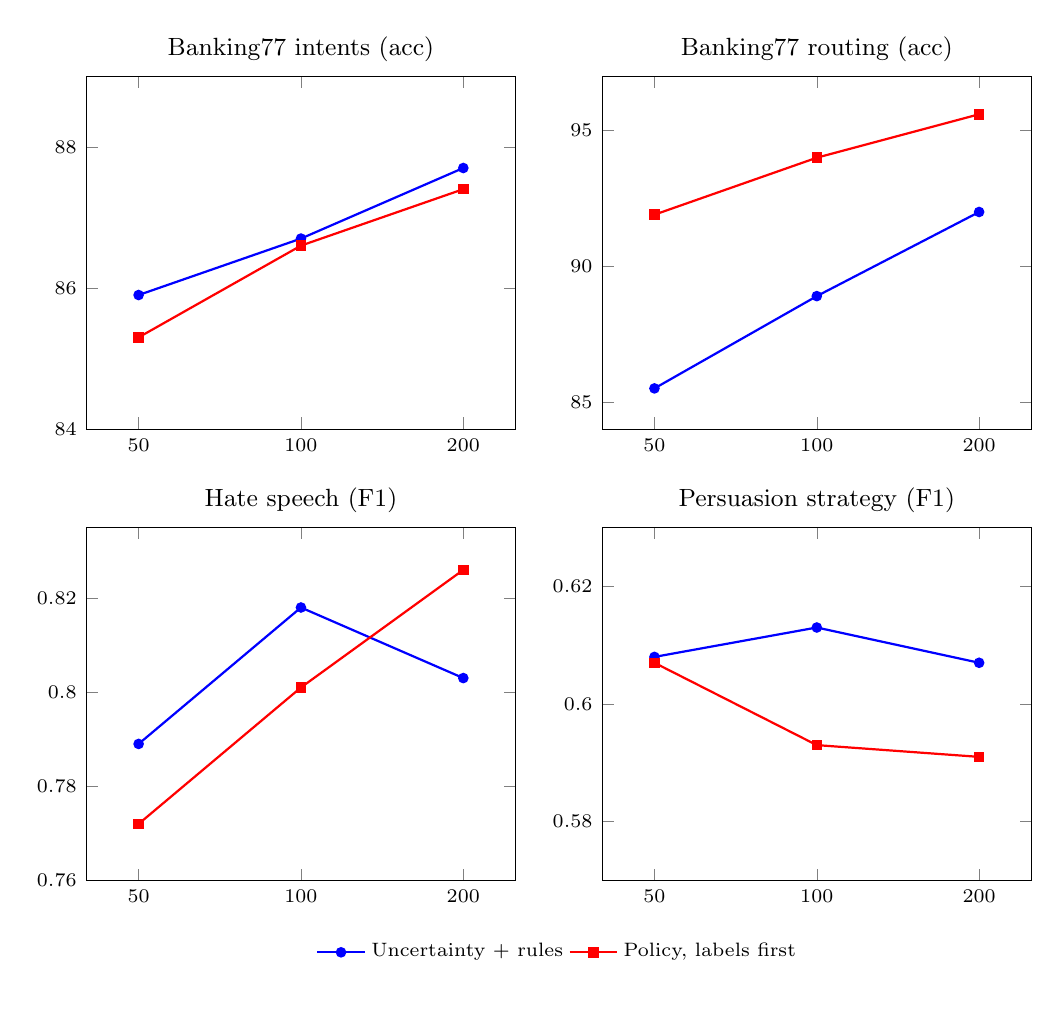
\begin{tikzpicture}
\begin{groupplot}[group style={group size=2 by 2, horizontal sep=1.1cm, vertical sep=1.25cm},
  width=0.58\linewidth, height=0.5\linewidth, xmode=log, log basis x=2, xtick={50,100,200},
  xticklabels={50,100,200}, xmin=40, xmax=250, tick label style={font=\scriptsize},
  title style={font=\small, yshift=-1ex}, every axis plot/.append style={thick, mark size=1.5pt}]
\nextgroupplot[title={Banking77 intents (acc)}, ymin=84, ymax=89,
  legend to name=budgetlegend, legend columns=2, legend style={font=\scriptsize, draw=none}]
\addplot[blue, mark=*] coordinates {(50,85.9) (100,86.7) (200,87.7)};
\addlegendentry{Uncertainty + rules}
\addplot[red, mark=square*] coordinates {(50,85.3) (100,86.6) (200,87.4)};
\addlegendentry{Policy, labels first}
\nextgroupplot[title={Banking77 routing (acc)}, ymin=84, ymax=97]
\addplot[blue, mark=*] coordinates {(50,85.5) (100,88.9) (200,92.0)};
\addplot[red, mark=square*] coordinates {(50,91.9) (100,94.0) (200,95.6)};
\nextgroupplot[title={Hate speech (F1)}, ymin=0.76, ymax=0.835, yticklabel style={/pgf/number format/fixed, /pgf/number format/precision=2}]
\addplot[blue, mark=*] coordinates {(50,0.789) (100,0.818) (200,0.803)};
\addplot[red, mark=square*] coordinates {(50,0.772) (100,0.801) (200,0.826)};
\nextgroupplot[title={Persuasion strategy (F1)}, ymin=0.57, ymax=0.63, yticklabel style={/pgf/number format/fixed, /pgf/number format/precision=2}]
\addplot[blue, mark=*] coordinates {(50,0.608) (100,0.613) (200,0.607)};
\addplot[red, mark=square*] coordinates {(50,0.607) (100,0.593) (200,0.591)};
\end{groupplot}
\node at ($(group c1r2.south)!0.5!(group c2r2.south)$) [yshift=-2.6em] {\pgfplotslegendfromname{budgetlegend}};
\end{tikzpicture}
\caption{mean final test score of three Opus runs at 50, 100 and 200 points. The 100-point values are the cells of Table 6.}
\label{fig:budget}
\end{figure}

\subsection{Other System 1 models}

\textbf{The classifiers transfer between System 1 models without retuning} (Table 8). The zero-shot classifiers spread by up to 0.07 macro-F1 across the four models, and no model is best on more than two tasks. Once Opus has written the definition from every label, the four models land within 0.031 macro-F1 of one another on every task and within one point on Banking77, and Jev, against which the classifiers were tuned, leads only on Banking77. A larger model adds little to a classifier that already states the definition: Sonnet 5 costs 40--75 times as much per record as Jev and is level with it.

\begin{table*}[t]
\centering\small\setlength{\tabcolsep}{3.5pt}
\begin{tabularx}{\textwidth}{lRRRRRRRR}
\toprule
Task & Zero-shot: Jev & Luna & Perplexity & Sonnet 5 & Opus, all labels: Jev & Luna & Perplexity & Sonnet 5 \\
\midrule
Banking77 intents (acc) & 80.2 & \textbf{82.8} & 79.3 & 81.2 & \textbf{91.9} & 91.5 & 91.1 & 91.0 \\
Banking77 routing (acc) & 73.7 & \textbf{77.6} & 72.6 & 76.5 & \textbf{97.5} & 96.5 & 96.6 & 96.7 \\
Hate speech (macro-F1) & \textbf{0.741} & 0.740 & 0.709 & 0.691 & 0.823 & \textbf{0.826} & 0.800 & 0.821 \\
Persuasion strategy (macro-F1) & 0.455 & 0.461 & 0.462 & \textbf{0.524} & 0.616 & \textbf{0.621} & 0.615 & 0.605 \\
Donation outcome (macro-F1) & \textbf{0.733} & 0.721 & 0.724 & 0.703 & 0.680 & 0.681 & 0.708 & \textbf{0.711} \\
Deal reached (macro-F1) & 0.889 & 0.899 & 0.896 & \textbf{0.905} & 0.896 & \textbf{0.912} & 0.906 & 0.896 \\
Cost per 1,000 records (USD) & 0.02--0.05 & 0.04--0.09 & 0.01--0.03 & 1.1--2.7 & 0.09--0.45 & 0.10--0.97 & 0.06--0.36 & 4.8--16.7 \\
\bottomrule
\end{tabularx}
\caption{the zero-shot and Opus all-labels classifiers, built against Jev and run unchanged on four System 1 models. Sonnet costs are at batch (half) price.}
\label{tab:8}
\end{table*}

The budgeted classifiers transfer at least as well (Table 9). Luna is within 0.003 of Jev on every task mean and matches or beats it in 10 of the 14 runs, and Perplexity's decision model is within 0.4 points of Jev on Banking77 and level with it or ahead on the conversation tasks, by up to 0.028 macro-F1 on hate speech. These classifiers were tuned on a few dozen labels rather than fitted option by option to Jev's answers on thousands of records, which may be why they lose nothing in transfer.

\begin{table*}[t]
\centering\small\setlength{\tabcolsep}{3.5pt}
\begin{tabularx}{\textwidth}{lRRRR}
\toprule
Task & Runs & Jev & Luna & Perplexity \\
\midrule
Banking77 intents (acc) & 3 & 87.3, 87.3, 85.8 (86.8) & 88.2, 87.9, 86.8 (\textbf{87.6}) & 87.5, 86.3, 85.4 (86.4) \\
Banking77 routing, free (acc) & 3 & 94.1, 92.1, 92.4 (92.8) & 94.3, 92.2, 92.9 (\textbf{93.1}) & 94.4, 92.2, 92.1 (92.9) \\
Hate speech (macro-F1) & 3 & 0.820, 0.779, 0.767 (0.789) & 0.809, 0.798, 0.776 (0.794) & 0.829, 0.822, 0.800 (\textbf{0.817}) \\
Persuasion strategy (macro-F1) & 3 & 0.589, 0.592, 0.629 (0.603) & 0.593, 0.592, 0.620 (0.602) & 0.611, 0.617, 0.616 (\textbf{0.615}) \\
Donation outcome, free (macro-F1) & 1 & \textbf{0.706} & 0.703 & \textbf{0.706} \\
Deal reached, free (macro-F1) & 1 & 0.873 & \textbf{0.880} & 0.873 \\
\bottomrule
\end{tabularx}
\caption{final classifiers of budgeted Opus builders, built against Jev and run unchanged on Luna and Perplexity's decision model. The runs are the uncertainty runs of the pilot on Banking77 intents, the policy-first runs of Table 6 on hate speech and persuasion strategy, and free-strategy runs on the other tasks, chosen before the full grid; we did not rescore the later runs. Means in parentheses.}
\label{tab:9}
\end{table*}

\subsection{Cost}

Building a classifier from a user interview with 100 points costs \$1.01--5.43 per run on average (Table 10), most of it the builder's own API calls and System 1 calls while building; the simulated user adds at most \$0.31 per run on average, and writing its note on how the labels apply the policy cost \$6--25 per task, once. Doubling the budget to 200 points triples the cost, mostly in System 1 calls on the larger set of bought labels. With every label, running drafts over thousands of records raises the System 1 cost of building to \$3--6 per run. Once built, the classifiers cost \$0.07--0.35 per 1,000 records with Jev, two to four times as much with Luna, and \$4.8--16.7 with Sonnet 5 even at batch price. Fine-tuning RoBERTa-base took from a minute to five hours on one M4 Max GPU, depending on the task. The runs reported in this paper cost about \$1,680 in API calls.

\begin{table*}[t]
\centering\small\setlength{\tabcolsep}{3.5pt}
\begin{tabularx}{\textwidth}{lRRRRRRR}
\toprule
Setting & Runs & Builder & Simulated user & System 1 while building & Total to build & Minutes & Final classifier, per 1,000 records \\
\midrule
Budgeted, Opus (cross-model) & 9 & 2.40 & 0.01 & 3.02 & 5.43 & 15.7 & 0.34 \\
Budgeted, Sonnet (cross-model) & 9 & 0.72 & 0.12 & 0.68 & 1.52 & 10.8 & 0.16 \\
Budgeted, Haiku (cross-model) & 9 & 0.47 & 0.28 & 0.25 & 1.01 & 9.0 & 0.07 \\
Budgeted, Opus (cross-strategy) & 90 & 1.58 & 0.31 & 1.44 & 3.34 & 11.7 & 0.24 \\
Budgeted, Opus, interview lean & 18 & 2.14 & 0.28 & 1.75 & 4.17 & 12.2 & 0.24 \\
Budgeted, Opus, rules only & 5 & 2.30 & --- & 3.07 & 5.37 & 12.7 & 0.35 \\
Budgeted, Opus, 50 points & 24 & 1.30 & 0.13 & 1.56 & 2.99 & 15.2 & 0.25 \\
Budgeted, Opus, 200 points & 24 & 3.10 & 0.20 & 6.26 & 9.55 & 58.3 & 0.42 \\
All labels, Opus & 6 & 1.93 & --- & 6.09 & 8.02 & 19.6 & 0.25 \\
All labels, Sonnet & 3 & 0.71 & --- & 3.14 & 3.85 & 8.7 & 0.12 \\
All labels, Haiku & 3 & 0.55 & --- & 5.06 & 5.61 & 11.7 & 0.12 \\
\bottomrule
\end{tabularx}
\caption{mean cost per run in USD. Builder is the agent's API cost; the simulated user is Claude Opus 5.5, and the rules-only runs asked it nothing; System 1 while building is the builder's Jev calls. The cross-model rows use the strategies chosen on validation, and the cross-strategy row covers every cell of Table 6 except the lean interview, which has its own row. The last column is the Jev cost of running the final classifier.}
\label{tab:10}
\end{table*}

\section{Discussion: monitoring and updating}

The experiments measure building, but System 2's job continues after a classifier is deployed. Its inputs drift, the user's definition changes, and errors surface that no building set contained. Three properties of NL classifiers make this part of the job tractable for an agent. First, monitoring can reuse the building strategies as sampling policies over the live stream: uncertainty sampling surfaces records near the decision boundary, a random audit estimates the current accuracy without bias, and running two versions side by side surfaces the records on which an edit would change the outcome. Our results suggest that no single policy is enough: on routing, a confidently wrong intent-to-team assignment never looks uncertain, so a monitor that only follows uncertainty would miss it, and an audit or a direct question would find it. Second, an update is an edit to a readable definition. When the user says that a kind of message now goes to another team, the agent changes one entry of the team map; a fine-tuned encoder would need labelled examples of the change and a retraining run before it applied the new rule. Third, the agent can judge its own classifier when it has a development set of a few hundred labels (\S{}6.1), which gives it a basis for deciding when to escalate to the user and when to stop. Measuring this loop, with drifting streams and users whose definitions change, is future work.

\section*{Limitations}

\textbf{The user is simulated.} Every answer comes from Claude Opus 5.5 holding the guideline, a note on how the labels apply it and a labelled sample, and Section 6.3 shows that what the simulated user knows changes which strategies win. A real user answers less consistently, may not know how their own labels apply the policy, and does not price questions by a fixed rubric. The simulated user is from the same model family as the builders, which may make its answers easier for them to use. We did not run a study with people.

\textbf{Strategy selection is noisy.} We choose each task's strategy on a validation split of 100 to 224 records, and the strategies often differ by less than the spread between runs of one strategy. Validation and test agree on four of six tasks, and where they disagree the cost is small, but the ranking of close strategies should not be read as settled. The pilot, which narrowed the strategies we tried, compared them on test, and the transfer runs of Table 9 were chosen before the full grid. With three runs per cell, a permutation test over runs cannot go below p = 0.05, and the all-labels results are single runs.

\textbf{The tasks are few and public.} We study six English tasks with one System 1 model used while building. Five come from public corpora that the builders may have seen in training; routing, whose mapping is our own, is the only task where the definition cannot have been memorised. Our hate speech splits are drawn from the official test set and are not comparable with published results.

\textbf{The harness had faults.} Until we found it, a crash in the hook that checks each tool call let calls whose arguments it could not parse run unchecked: 511 of 8,790 tool calls in 188 runs. We read every one of them, and none touched the labelled data, the task files or another run. Seven runs that failed on network errors were rerun from scratch. Some runs that only bought labels were kept from earlier rounds with an earlier simulated user, since label requests return the same gold labels under every version.

\bibliography{references}

\end{document}
